%%% License: Creative Commons Attribution Share Alike 4.0 (see https://creativecommons.org/licenses/by-sa/4.0/)

\documentclass[english,10pt
,aspectratio=169
%,handout
%,notes
]{beamer}
%%% License: Creative Commons Attribution Share Alike 4.0 (see https://creativecommons.org/licenses/by-sa/4.0/)

\DeclareGraphicsExtensions{.eps, .pdf,.png,.jpg,.mps,}
\usetheme{reMedian}
\usepackage{parskip}
\makeatother

\renewcommand{\baselinestretch}{1.1} 

\usepackage{amsmath, amssymb, amsfonts, amsthm}
\usepackage{enumerate}
%\usepackage{enumitem}
\usepackage{hyperref}
\usepackage{url}
\usepackage{bbm}
\usepackage{color}

\usepackage{tikz}
\usepackage{tikzscale}
\newcommand*\circled[1]{\tikz[baseline=(char.base)]{
		\node[shape=circle,draw, inner sep=-20pt] (char) {#1};}}
\usetikzlibrary{automata,positioning}
\usetikzlibrary{decorations.pathreplacing}
\usepackage{pgfplots}
\usepgfplotslibrary{fillbetween}
\usepackage{graphicx}

\usepackage{setspace}
\thinmuskip=1mu
\medmuskip=1mu 
\thickmuskip=1mu 


\usecolortheme{default}
\usepackage{verbatim}
\usepackage[normalem]{ulem}

\usepackage{apptools}
\AtAppendix{
	\setbeamertemplate{frame numbering}[none]
}
\usepackage{natbib}


% red strikeout
\newcommand\soutred{\bgroup\markoverwith
	{\textcolor{red}{\rule[0.55ex]{2pt}{0.8pt}}}\ULon}



% To use LyX frames from old version:
\def\lyxframeend{} % In case there is a superfluous frame end
\long\def\lyxframe#1{\@lyxframe#1\@lyxframestop}%
\def\@lyxframe{\@ifnextchar<{\@@lyxframe}{\@@lyxframe<*>}}%
\def\@@lyxframe<#1>{\@ifnextchar[{\@@@lyxframe<#1>}{\@@@lyxframe<#1>[]}}
\def\@@@lyxframe<#1>[{\@ifnextchar<{\@@@@@lyxframe<#1>[}{\@@@@lyxframe<#1>[<*>][}}
\def\@@@@@lyxframe<#1>[#2]{\@ifnextchar[{\@@@@lyxframe<#1>[#2]}{\@@@@lyxframe<#1>[#2][]}}
\long\def\@@@@lyxframe<#1>[#2][#3]#4\@lyxframestop#5\lyxframeend{%
	\frame<#1>[#2][#3]{\frametitle{#4}#5}}


\title{Mechanism Design}

\subtitle{8: Communication with verifiable information}

\author{Egor Starkov}

\date{K{\o}benhavns Unversitet \\
	Fall 2022}


\begin{document}
	\AtBeginSection[]{
		\frame{
			\frametitle{This slide deck:}
			\tableofcontents[currentsection,currentsubsection]
	}}
	\frame[plain]{\titlepage}



\begin{frame}{Introduction}
\begin{itemize}
	\item Throughout the course we dealt with situations where players had some private information that the designer was interested in.
	\item The players could act based on this private info, but had no way of proving their type (except through the choice of actions).
	\item Would anything change if the players could \alert{disclose hard evidence} of their type?
	\item This lecture is based on (and expands on) the address by \cite{dekel_evidence_2016}.
	\item For a broader survey of the literature, see the survey by \cite{dranove_quality_2010}.
\end{itemize}
\end{frame}


\begin{frame}{Hard evidence}
	Examples of hard (verifiable) evidence:
	\begin{itemize}
		\item statements about \structure{verifiable characteristics of the product}:
		\begin{itemize}
			\item performance, 
			\item energy efficiency for appliances / fuel efficiency for vehicles,
			\item university departments disclose graduates' employability data.
		\end{itemize}
		\item \structure{external ratings and certificates} 
		\begin{itemize}
			\item cafes \& restaurants have sanitary ratings
			\item exchange-traded firms get credit ratings
			\item videogames and movies get age ratings, and also critics' reviews
		\end{itemize}
	\end{itemize}
\end{frame}


\section{Disclosure games}

\begin{frame}{Disclosure games: basic version \citep{grossman_informational_1981}}
	Let's start with \alert{disclosure games}: no design, simply an exploration of how the sender would behave.
	\begin{enumerate}[<+->]
		\item A firm has a product of privately known quality $\theta \in \Theta \equiv \{\underline{\theta}, ..., \bar{\theta}\}$, chooses whether to show a certificate that verifies $\theta$.
		
		\item A consumer observes evidence (if any) and updates their belief $\phi_c \in \varDelta(\Theta)$.
		
		\item The firm's payoff is $\mathbb{E}[\theta | \phi_c]$.
		\begin{itemize}
			\item I.e., the firm wants to induce the highest possible belief (so it can charge higher price, get more consumers, etc -- not modelled)
		\end{itemize}
	\end{enumerate}
\end{frame}


\begin{frame}{Unraveling}
	\begin{theorem}[Unraveling]
		In equilibrium, all firm types $\theta$ present evidence, so there is full learning.
	\end{theorem}
	\begin{itemize}[<+->]
		\item Suppose not: there is a set of types $\Theta_S$ that stay silent (do not show evidence).
		\item Then the firm's payoff when hiding evidence is $\mathbb{E}[\theta | \phi_0, \theta \in \Theta_S]$, where $\phi_0$ is the consumer's prior belief.
		\item Consider type $\bar{\theta}_S \equiv \max \Theta_S$. Revealing the type (with evidence) yields payoff $\bar{\theta}_S$, which is higher than the payoff from silence (which is a weighted average of $\bar{\theta}_S$ and lower types).
		\item So regardless of which types stay silent, the highest of such types would like to separate. Then the highest of the remaining types would like to do the same, etc -- this process is called \alert{unraveling}.
	\end{itemize}
\end{frame}


\begin{frame}{Unraveling: reasons and robustness}
	\begin{itemize}
		\item The opportunity to present evidence leads to \structure{all information being revealed}.
		\item Note the buyer-designer would \alert{not be able} to get this result \alert{without evidence}:
		\begin{itemize}
			\item As we discussed, our elicitation methods relied on different agent types $\theta$ having different preferences (e.g., single-crossing preferences over multidimensional outcomes, non-monotone preferences over one-dimensional outcome).
			
			\item In this example, only the buyer's preferences depend on the type (or so the story suggests) -- note that the firm gets $\mathbb{E}[\theta | \phi_c]$ regardless of true $\theta$ -- so all types $\theta$ have the exact same reporting incentives! 
		\end{itemize}
		\pause
		\item The result works for interval $\Theta$ too, though the argument is slightly more subtle. 
		\item \cite{milgrom_good_1981} showed unraveling works in a more general version, where the firm can show evidence for any subset of $\Theta$ that it belongs to.
		\item We will now look at a couple of variations where unraveling \alert{breaks}.
	\end{itemize}
\end{frame}


\section{Disclosure games: variations}

\begin{frame}{Costs of disclosure \citep{verrecchia_discretionary_1983}}
\begin{columns}
	\begin{column}{0.6\linewidth}
		{\setstretch{1.3}
			\begin{itemize}
				\item Continue the previous example, but suppose now that showing evidence costs $c > 0$ for the firm.
				
				\item Then for the low enough types, the profit from showing evidence is not worth the cost.
				
				\pause 
				\item \textbf{Graph:} $\theta \sim U[0,1]$. Start with no one revealing. Then $\theta=1$ wants to reveal, payoff increases from $\mathbb{E}[\theta]=0.5$ to $1-c$. Same (iteratively) for all high-ish $\theta$s up to $\theta = 2c$, who is exactly indifferent: $\mathbb{E}[\theta | \theta < 2c] = c = \theta-c$. So all types $\theta \in [0,2c]$ pool together in silence.
			\end{itemize}
		}
	\end{column}
	\begin{column}{0.4\linewidth}
		%\pause[1]
		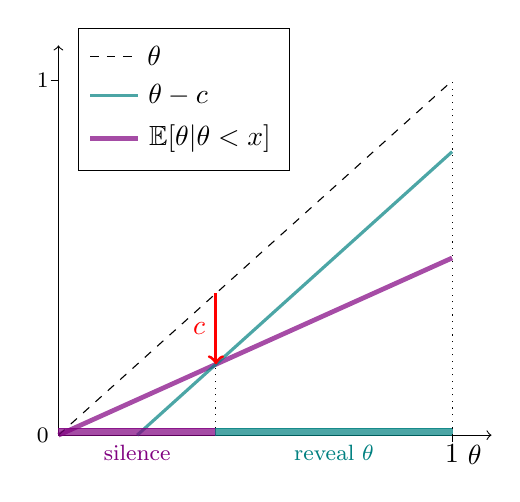
\begin{tikzpicture}[xscale=5,yscale=4.5]
			\draw[->] (0,0) -- (1.1,0) node[below left]{$\theta$};
			\draw[->] (0,0) -- (0,1.1);
			\draw (0,0) node[left]{\footnotesize $0$};
			
			% Plot
			\draw[line width=0.6mm, violet, opacity=0.7] (0,0) -- (1,0.5);
			\draw[dashed] (0,0) -- (1,1);
			\draw[line width=0.4mm, teal, opacity=0.7] (0.2,0) -- (1,0.8);
			\draw[line width=0.4mm, red, <-] (0.4,0.2) -- (0.4,0.3) node[left]{$c$} -- (0.4,0.4);
			\draw[dotted] (0.4,0) -- (0.4,0.2);
			
			\filldraw[violet, opacity=0.7] (0,0) -| (0.4,0.02) -| (0,0);
			\draw (0.2,0) node[below, violet]{\footnotesize silence};
			\filldraw[teal, opacity=0.7] (1,0) -| (0.4,0.02) -| (1,0);
			\draw (0.7,0) node[below, teal]{\footnotesize reveal $\theta$};
			
			% Ticks
			% x axis
			\draw (1,0) coordinate(q3) node[below]{$1$};
			\draw (q3) ++(0,-0.02) -- ++(0,0.02);
			\draw[dotted] (1,0) -- (1,1);
			
			% y axis
			\draw (0,1) coordinate(u2) node[left]{\footnotesize $1$};
			\draw (u2) ++(-0.02,0) -- ++(0.02,0);
			%\draw[dotted] (u2) -- (1,1);
			
			%Legend
			\matrix [draw, fill=white, below right] at (0.05,1.15) {
				\draw [dashed] ++(-0.3,0) -- ++(0.6,0) node[black,right] {$\theta$}; \\
				\draw [line width=0.4mm, teal, opacity=0.7] ++(-0.3,0) -- ++(0.6,0) node[black,right, opacity=1] {$\theta-c$}; \\
				\draw [line width=0.6mm, violet, opacity=0.7] ++(-0.3,0) -- ++(0.6,0) node[black,right,opacity=1] {$\mathbb{E}[\theta | \theta<x]$}; \\
			};
		\end{tikzpicture}
	\end{column}
\end{columns}
\end{frame}


\begin{frame}{Uncertain evidence \citep{dye_disclosure_1985,jung_disclosure_1988}}
\begin{itemize}
	\item Now return to the case $c=0$, but the firm only has \structure{evidence with probability $\lambda < 1$}.
	\item With probability $1-\lambda$ the firm has no evidence and is forced to stay silent.
	\item Then, if types $\Theta_S$ stay silent:
	\begin{align*}
		\mathbb{E}[\theta \mid \text{silence}] = \frac{\lambda \mathbb{P}(\Theta_S) \mathbb{E}[\theta \mid \theta \in \Theta_S] + (1-\lambda) \mathbb{E}[\theta]}{\lambda \mathbb{P}(\Theta_S) + (1-\lambda)} > \mathbb{E}[\theta \mid \theta \in \Theta_S].
	\end{align*}
	The consumer is not as pessimistic after no disclosure (as when $\lambda=1$), because they understand the firm may not have any evidence. So profit from disclosure is smaller.
	\item This may again lead to some low types staying silent (pretending to have no evidence).
\end{itemize}
\end{frame}


\begin{frame}{Uncertain evidence: example}
\begin{columns}
	\begin{column}{0.6\linewidth}
		{\setstretch{1.3}
			\begin{itemize}
				\item Suppose again $\theta \sim U[0,1]$ and let $\lambda = 3/4$.
				\item \textbf{Conjecture:} in eqm, types $\theta \in [x,1]$ disclose their type if they can; types $\theta \in [0, x)$ always silent. Then 
				\pause
				\begin{align*}
					\mathbb{E}[\theta \mid \text{silence}] 
					%= \frac{\lambda \mathbb{P}(\Theta_S) \mathbb{E}[\theta \mid \theta \in \Theta_S] + (1-\lambda) \mathbb{E}[\theta]}{\lambda \mathbb{P}(\Theta_S) + (1-\lambda)} 
					%= \frac{\frac{3}{4} \cdot x \cdot \frac{x}{2} + \frac{1}{4} \cdot \frac{1}{2}}{\frac{3}{4} \cdot x + \frac{1}{4}} 
					= \frac{3x^2 + 1}{2(3x + 1)}
				\end{align*}
				\item Type $\theta$ discloses if $\theta \geq \mathbb{E}[\theta \mid \text{silence}]$ and silent otherwise. Hence $x = \mathbb{E}[\theta \mid \text{silence}] \iff x=1/3$.
				\item So there is an eqm, where types $\theta \in [1/3,1]$ disclose their type if they can; types $\theta \in [0, 1/3)$ always stay silent. (Can verify that it is unique.)
			\end{itemize}
		}
	\end{column}
	\begin{column}{0.4\linewidth}
		%\pause[1]
		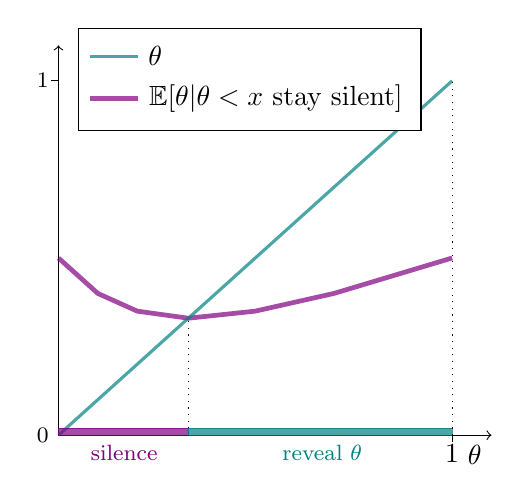
\begin{tikzpicture}[xscale=5,yscale=4.5]
			\draw[->] (0,0) -- (1.1,0) node[below left]{$\theta$};
			\draw[->] (0,0) -- (0,1.1);
			\draw (0,0) node[left]{\footnotesize $0$};
			
			% Plot
			\draw[line width=0.6mm, violet, opacity=0.7, smooth] (0,0.5) -- (0.1,0.4) -- (0.2,0.35) -- (0.33,0.33) -- (0.5,0.35) -- (0.7,0.4) -- (1,0.5);
			\draw[line width=0.4mm, teal, opacity=0.7] (0,0) -- (1,1);
			\draw[dotted] (0.33,0) -- (0.33,0.33);
			
			\filldraw[violet, opacity=0.7] (0,0) -| (0.33,0.02) -| (0,0);
			\draw (0.167,0) node[below, violet]{\footnotesize silence};
			\filldraw[teal, opacity=0.7] (1,0) -| (0.33,0.02) -| (1,0);
			\draw (0.67,0) node[below, teal]{\footnotesize reveal $\theta$};
			
			% Ticks
			% x axis
			\draw (1,0) coordinate(q3) node[below]{$1$};
			\draw (q3) ++(0,-0.02) -- ++(0,0.02);
			\draw[dotted] (1,0) -- (1,1);
			
			% y axis
			\draw (0,1) coordinate(u2) node[left]{\footnotesize $1$};
			\draw (u2) ++(-0.02,0) -- ++(0.02,0);
			%\draw[dotted] (u2) -- (1,1);
			
			%Legend
			\matrix [draw, fill=white, below right] at (0.05,1.15) {
				\draw [line width=0.4mm, teal, opacity=0.7] ++(-0.3,0) -- ++(0.6,0) node[black,right, opacity=1] {$\theta$}; \\
				\draw [line width=0.6mm, violet, opacity=0.7] ++(-0.3,0) -- ++(0.6,0) node[black,right,opacity=1] {$\mathbb{E}[\theta | \theta < x \text{ stay silent}]$}; \\
			};
		\end{tikzpicture}
	\end{column}
\end{columns}
\end{frame}


\begin{frame}{Disclosure games: conclusion}
\begin{itemize}
	\item In the basic game with evidence, unraveling leads to \structure{full information revelation}.
	\item Unraveling can be tamed with disclosure costs or receivers allowing for a chance of sender having no evidence. (There are, of course, not the only reasons; see \cite{dranove_quality_2010} for more.)
	\item Even in those later cases, the idea is simple: \structure{reveal good news}, \alert{hide bad news}.
	\item Think of this as an additional tool in your information extraction toolbox.
\end{itemize}
\end{frame}


\begin{frame}{Good news and bad news}
	The asymmetry between \textbf{good \& bad news} is fun to explore:
	\begin{itemize}[<+->]
		\item it means that \alert{silence is bad news} (but humans are bad at inferring it, see \cite*{jin_is_2021}), 
		\item that \alert{silence leaves more uncertainty} than good announcements \citep{shin_disclosures_2003}, 
		\item that bad news are revealed in \alert{bunches} \citep*{acharya_endogenous_2011}
		\item that the desire to have good news to disclose leads to \alert{excessive risk-taking} \citep*{ben-porath_disclosure_2018} %\alert{excessive information acquisition} and 
		
		\bigskip 
		\item There are also a few reasons why sender might want to hide good news, see an overview in \cite{smirnov_bad_2022}
	\end{itemize}
\end{frame}


\begin{frame}{A word from our sponsor}
\begin{itemize}
	\item As usual, \textbf{dynamic disclosure games} are also extremely fun (with evidence arriving over time and sender choosing what/when to disclose), but we won't talk about those. Instead... 
\end{itemize}
\end{frame}


\section{Mechanism design with evidence}

\begin{frame}{Multiple players}
\begin{itemize}
	\item With multiple senders (who have access to the same evidence and opposed interests), can get full info even when individual sender only shows partial evidence \citep{milgrom_relying_1986} -- this strengthens the results we had without evidence
	\item A weaker version is proved by ... %TODO
\end{itemize}
\end{frame}


\begin{frame}{Item allocation with evidence}
\begin{itemize}
	\item \cite{ben-porath_mechanisms_2019} consider an item allocation problem where %TODO
\end{itemize}
\end{frame}


\appendix
\begin{frame}[allowframebreaks]{References}
\bibliography{teaching}
\bibliographystyle{abbrvnat}
\end{frame}


\end{document}